\documentclass[xcolor=dvipsnames, USenglish]{beamer}  %notes=show to print them in the generated pdf
% Packages for a reasonable beamer session
\usepackage[T1]{fontenc}
\usepackage[ansinew]{inputenc}
\usepackage{textcomp}
\usepackage{lmodern}
\usepackage{csquotes}
\usepackage{babel}

\usepackage{graphicx}

\usepackage{amsmath}
\usepackage{amsfonts}
\usepackage{amssymb}
\usepackage{amsthm}
\usepackage{bm}

\usepackage{booktabs}
\usepackage{tabularx}

\usepackage{hyperref}

\usepackage{ellipsis}

% Additional packages
\usepackage{graphicx}
\usepackage{subfigure}
\usepackage{xcolor}


\usepackage[style=authoryear, backend=biber]{biblatex}
\setbeamertemplate{itemize/enumerate body begin}{\setlength{\leftmargini}{1.5em}}
\renewcommand*{\nameyeardelim}{\addcomma\addspace}
\addbibresource{\jobname.bib}
\renewcommand{\footnotesize}{\tiny}

\usepackage{tikz,pgf,calc}
%\usetikzlibrary{matrix, shapes, positioning, calc,
%  decorations.pathreplacing, shapes.geometric, arrows}
\usetikzlibrary{shapes.geometric, arrows, calc}
\tikzstyle{startstop} = [rectangle, rounded corners, minimum width=3cm, minimum height=1cm, text centered, text width=1.5cm, draw=black, fill=red!30]
\tikzstyle{io} = [trapezium, trapezium left angle=70, trapezium right angle=110, minimum width=3cm, minimum height=1cm, text centered, draw=black, fill=blue!30]
\tikzstyle{process} = [rectangle, minimum width=3cm, minimum height=1cm, text centered, draw=black, fill=orange!30]
\tikzstyle{decision} = [diamond, minimum width=3cm, minimum height=0.5cm, text centered, draw=black, fill=green!30]
\tikzstyle{arrow} = [thick,->,>=stealth]

%% References
\newlength\leftsidebar
\makeatletter
\setlength\leftsidebar{\beamer@leftsidebar}
\makeatother

\usepackage[absolute,overlay]{textpos}
\newenvironment{reference}[2]{%
  \begin{textblock*}{\textwidth}(\leftsidebar+#1,\paperheight-#2)
      \scriptsize\bgroup\color{red!50!black}}{\egroup\end{textblock*}}

% Path to graphics
\graphicspath{{../img/}}

% Sources
\usepackage{setspace}
\newcommand{\source}[1]{\begin{spacing}{0.5}{\fontsize{5}{6}\selectfont source: \itshape {#1}}\end{spacing}}
 % PACKAGES
% Collection of useful mathematical symbols and commands
% Calculus
\newcommand{\ud}{\mathrm{d}}
\newcommand{\pder}[2]{\frac{\partial{#1}}{\partial{#2}}}
\newcommand{\dpder}[2]{\frac{\partial^2{#1}}{\partial{#2^2}}}
\newcommand{\sderp}[3]{\frac{\partial^2{#1}}{\partial{#2}\partial{#3}}}
\newcommand{\tder}[2]{\frac{\ud{#1}}{\ud{#2}}}
\newcommand{\rot}[1]{\nabla \times {#1}}
\newcommand{\diver}[1]{\nabla \cdot {#1}}
\newcommand{\definter}[4]{\int_{#1}^{#2} {#3}\ud {#4}}
\newcommand{\inter}[2]{\int {#1}\ud {#2}}
\newcommand{\braket}[2]{\langle {#1} , {#2} \rangle}
% Misc
\newcommand{\eval}[1]{\Big |_{#1}}
\newcommand{\bset}[1]{\big\lbrace {#1} \big\rbrace}
\newcommand{\stimes}[2]{{#1}\!\times\!{#2}}
\newcommand{\trp}{\top}
\newcommand{\preup}[2]{{}^{#2}\!{#1}}

% Operators
\DeclareMathOperator*{\armin}{arg\,min}
\DeclareMathOperator*{\armax}{arg\,max}
\DeclareMathOperator*{\rank}{rank}
\DeclareMathOperator*{\cov}{cov}
\DeclareMathOperator*{\nullsp}{null}
% Logicals
\newcommand{\suchthat}{\big \backslash \;}
   % SYMBOLS

% ----------- extra packages
\usepackage{../beamer_themes/beamerthemeEawag_blue} % Eawag style

% ----------- Extra symbols
\newcommand{\ccov}[1]{{\color{red}k}\left(#1\right)}
\newcommand{\cmean}[1]{{\color{blue}m}\left(#1\right)}
\newcommand{\sm}{\scalebox{0.5}{-1}}

% ----------- For boxed equations
\usepackage{amsmath}
\usepackage{empheq}
\usepackage[most]{tcolorbox}
\newtcbox{\mymath}[1][]{%
    nobeforeafter, math upper, tcbox raise base,
    enhanced, colframe=blue!30!black,
    colback=blue!30, boxrule=1pt,
    #1}



%----------------
% title information
\title{Master Thesis - Final Presentation}
\subtitle{Applications of Emulation to the Hydrology Field\\\textcolor{Red}{not really just hydrology, e.g. weir equation}}
\author[\texttt{sebastiano.rusca@eawag.ch}]{Sebastiano Rusca}
\institute[Eawag]{Eawag: Swiss Federal Institute of Aquatic Science
  and Technology}
\date[12.03.2018]{March 12, 2018}

% Title suggestions
% * use an active title: with a verb, or using "in", not "application of ... to ..."
% * not a too bombastic one, "Emulation in hydrology" is too much
% * try to use "shallow water equation", this is what we actually emulate
% * first steps towards ...
% * a guide to emulation in ...


% ====================================================================

\begin{document}
%%%%%%%%%%%%%%%%%%%%%%%%%%%%%%%%%%%%%%%%%%%%%%%%%%%%%%%%%%%%%%%%%%%%%%%%%%%%%%%%
% CODE
\definecolor{bg}{rgb}{0.95,0.95,0.95}

\defverbatim[colored]\QinCode{
\begin{minted}[fontsize=\scriptsize, 
               numbersep=8pt,
               gobble=4,
               frame=lines,
               bgcolor=bg,
               framesep=2mm]{octave}

      nQ = 25; # number of experiments
      Qin = linspace (0.1, 10, nQ); # Qin values [m3/s]

\end{minted}
}

%%%%%%%%%%%%%%%%%%%%%%%%%%%%%%%%%%%%%%%%%%%%%%%%%%%%%%%%%%%%%%%%%%%%%%%%%%%%%%%%
% ----------------
% Title frame
% load background for title
\setbeamertemplate{background}{
  \includegraphics[width=\paperwidth,height=\paperheight]
  {../beamer_themes/background_title_blue.png}}
{ \setbeamertemplate{footline}{} % no footer on title
  \begin{frame}
    \titlepage
  \end{frame}
}
% load background for all other slides
\setbeamertemplate{background}{
\includegraphics[width=\paperwidth,height=\paperheight]
{../beamer_themes/background_slides_blue.png}}
\setbeamertemplate{footline}[Sebastiano Rusca] % set footer
\addtocounter{framenumber}{-1}  % don't count title page

%%%%%%%%%%%%%%%%%%%%%%%%%%%%%%%%%%%%%%%%%%%%%%%
%----------------
\section{Introduction}

  \begin{frame}
    \frametitle{Outline}
    \begin{itemize}
      \item Master thesis goals
      \item What is emulation?
      \item Case studies
      \begin{itemize}
      %\itemsep0em
        \item A mechanistic emulator: \emph{fitting the weir equation}
        \item A hydrological emulator: \emph{estimating the time-to-threshold}
      \end{itemize}
      \item Conclusions
      \item Outlook
     \end{itemize}
  \end{frame}

% "learning the weir equation" or "fitting the weir equation", depends on what is actually presented

%%%%%%%%%%%%%%%%%%%%%%%%%%%%%%%%%%%%%%%%%%%%%%%%%%%%%%%%%%%%%%%%%%%%%%%%%%%%%%%%
% MASTER THESIS GOALS
  \begin{frame}
    \frametitle{Master thesis goals}
    \begin{itemize}
      \item Get an overview of emulation
      \begin{itemize}
        \item Learn about \emph{interpolation}, \emph{intrapolation} and \emph{extrapolation}
        \item Learn about \emph{Gaussian Processes}
      \end{itemize}
      \item Find an appropriate \emph{open source} hydrological simulator
      \begin{itemize}
      %\itemsep0em
        \item Learn its \emph{functioning} and \emph{customize} it for the required scope
        \item Produce \emph{test datasets} usable for emulation
      \end{itemize}
      \item Perform emulation with a \emph{didactic} example
      \begin{itemize}
      %\itemsep0em
        \item Mechanistic emulator: \emph{the weir equation}
      \end{itemize}
      \item Perform emulation in an \emph{hydrological} context
      \begin{itemize}
      %\itemsep0em
        \item Hydrological emulator: \emph{time-to-threshold}
      \end{itemize}
      \item Draw conclusions about emulation potential, especially applied to the \emph{hydrology},
            \emph{urban water} and \emph{water management} fields
    \end{itemize}
  \end{frame}


%%%%%%%%%%%%%%%%%%%%%%%%%%%%%%%%%%%%%%%%%%%%%%%%%%%%%%%%%%%%%%%%%%%%%%%%%%%%%%%%
% WHAT IS EMULATION?


%%%%%%%%%%%%%%%%%%%%%%%%%%%%%%%%%%%%%%%%%%%%%%%%%%%%%%%%%%%%%%%%%%%%%%%%%%%%%%%%
% CASE STUDY 1: OVERVIEW
\section{Case study 1: weir equation}

  \begin{frame}
    \frametitle{Mechanistic emulator: \emph{the weir equation}}
    \textbf{Goal}: fit the weir equation to simulated data\\
    \vfill
    \begin{alertblock}{Weir equation}
      \setlength\abovedisplayskip{0pt}
      \begin{equation*}
        Q = \frac{2}{3}\: \textcolor{red}{\mu}\: B_w\: \sqrt{2g}\: h_w^{\textcolor{red}{a}},
        \quad usu.\: \textcolor{red}{a = 3/2}
      \end{equation*}
    \end{alertblock}
    \vfill
    \centering
    $\boldsymbol{\mu :\,}$ \raisebox{-.2\height}{\includegraphics[width=0.8\textwidth]{img/weir_coefficients.png}}
    \source{Boes, Robert. "Wasserbau - Vorlesungsmanuskript." ETH Z\"urich - VAW, 2016.}
  \end{frame}
% * In this first case study we want to fit the weir equation to simulated data.
% * In a while we will see what relation this has with emulation and machine learning.
% * The weir equation can be derived analytically by assuming no friction losses and 
%   a uniform velocity distribution.
% * Results obtained are for a theoretical discharge, which diverges from empirical results, where
%   the assumption mentioned don't hold.
% * In order to obtain actual discharge a correction factor \mu has to be taken into account.
% * \mu is dependent on the type and shape of weir (broad-crested/narrow-crested) and which
%   particular shape.
% * To obtain the value of this coefficient the equation has to be fitted to 
%   experimental data.
% * Here below some \mu-values for some weir types are shown


%%%%%%%%%%%%%%%%%%%%%%%%%%%%%%%%%%%%%%%%%%%%%%%%%%%%%%%%%%%%%%%%%%%%%%%%%%%%%%%%
% CASE STUDY 1: STUDY SET-UP
  \begin{frame}
    \frametitle{Experiment overview}
    \textbf{Input discharge}
    \QinCode
    \vfill
    \textbf{Channel set-up}

    \centering
    \includegraphics[width=0.8\textwidth]{img/weir.png}
  \end{frame}


%%%%%%%%%%%%%%%%%%%%%%%%%%%%%%%%%%%%%%%%%%%%%%%%%%%%%%%%%%%%%%%%%%%%%%%%%%%%%%%%
% CASE STUDY 1: SIMULATIONS RESULTS
  \begin{frame}
    \frametitle{Simulation results}
    \begin{minipage}{.5\textwidth}
      \centering
      \small{Experiments free-surfaces}\\
      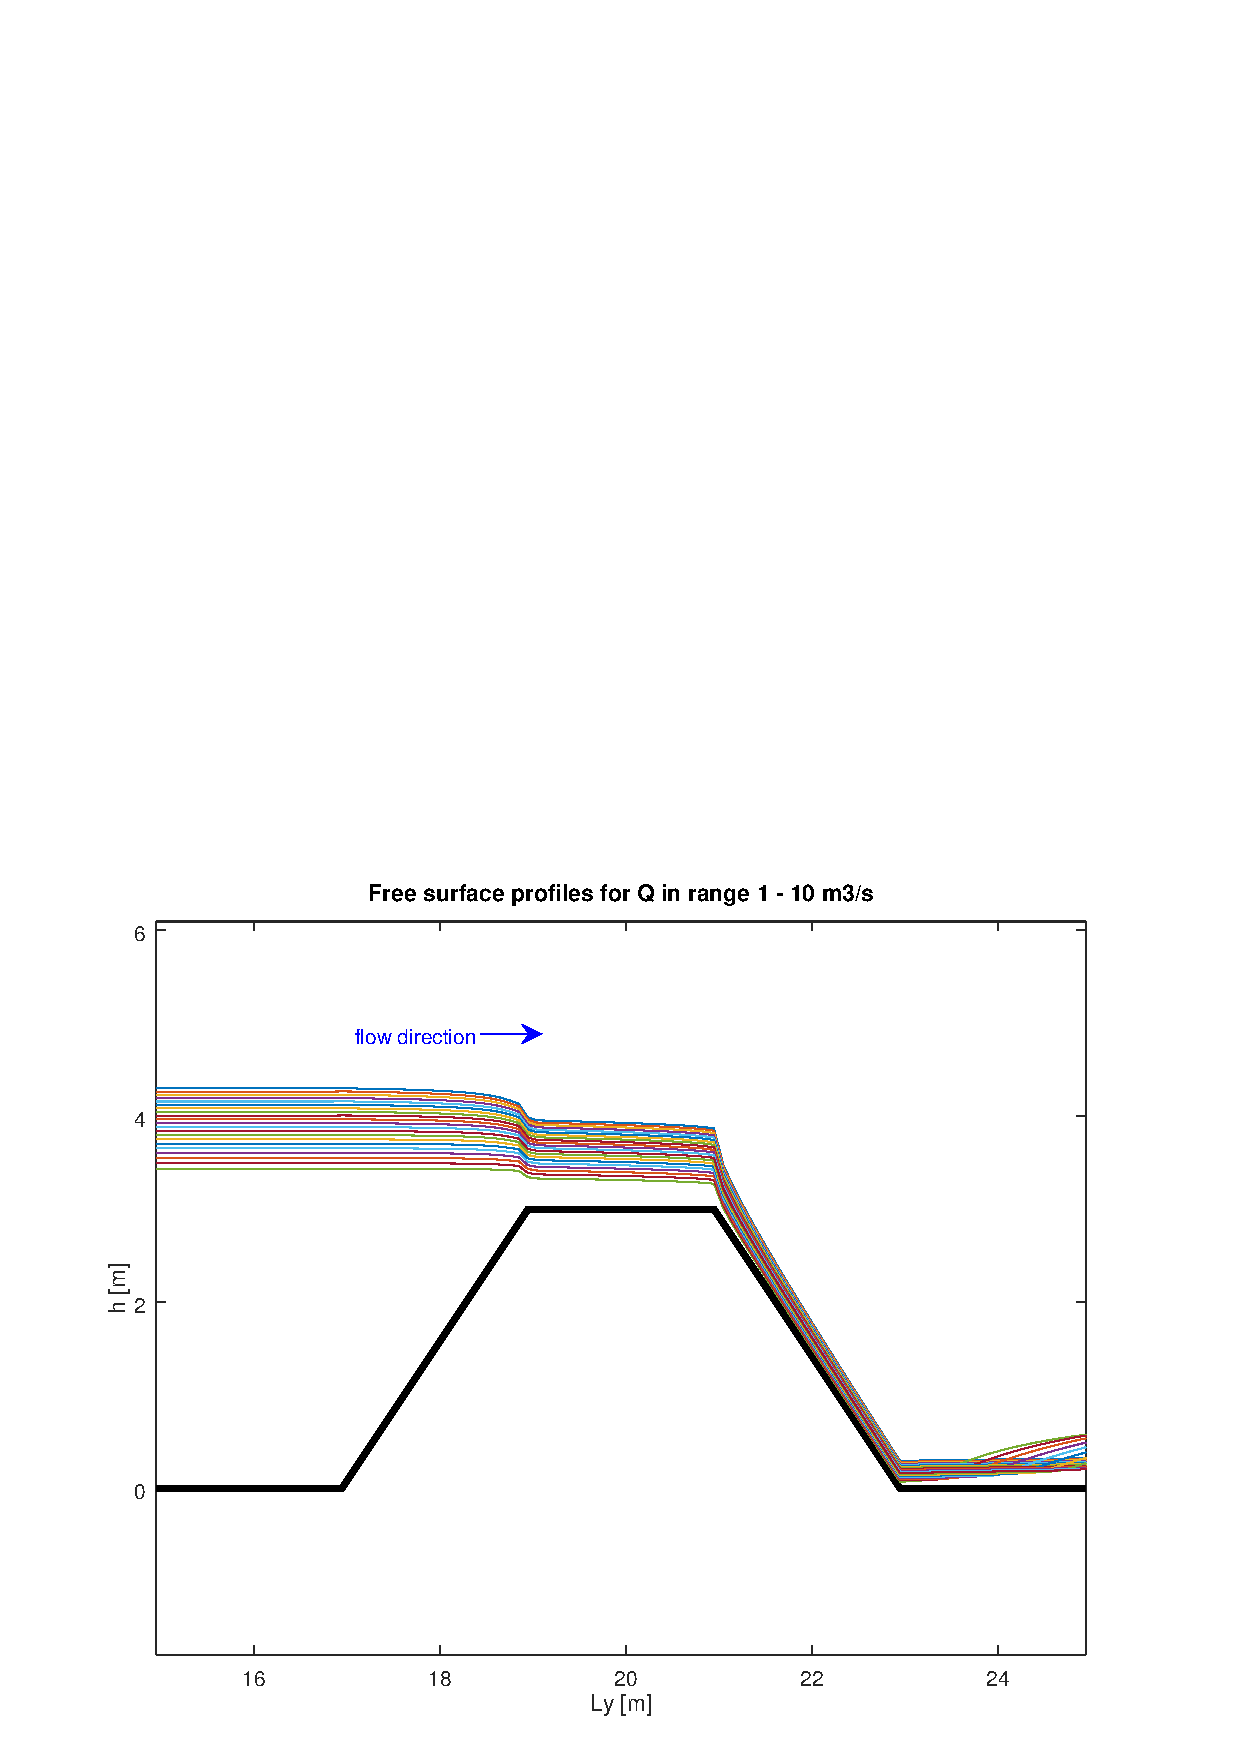
\includegraphics[width=\textwidth]{img/free_surfaces.png}
    \end{minipage}%
    \begin{minipage}{.5\textwidth}
      \centering
      \small{Experiments $h_w$ vs. $Q$}\\
      \includegraphics[width=\textwidth]{img/simulation_results.png}
    \end{minipage}
  \end{frame}


%%%%%%%%%%%%%%%%%%%%%%%%%%%%%%%%%%%%%%%%%%%%%%%%%%%%%%%%%%%%%%%%%%%%%%%%%%%%%%%%
% CASE STUDY 1: FITTING RESULTS
  \begin{frame}
    \frametitle{Fitting results}
    \begin{minipage}{.5\textwidth}
      \centering
      \small{Different fittings}\\
      \includegraphics[width=\textwidth]{img/fitting_results.png}
    \end{minipage}%
    \begin{minipage}{.5\textwidth}
      \centering
      \small{\emph{Model} vs. \emph{local} fitting}\\
      \includegraphics[width=\textwidth]{img/fitting_errors.png}
    \end{minipage}
  \end{frame}
% * 3 different fittings were done
% * Weir equation follows a power law, therefore the logarithm of the data was taken
%   and a linear regression was performed with all data.
%   values of \mu = 0.56 and a = 1.59 were found.
% * A linear interpolation was performed. performs very bad at the beginning (few points),
%   but quite good afterwards (almost overlaying).
% * A spline interpolation was performed. This performs good even between points
%   1 and 2 (almost overlaying).
% * I wanted to test the robustness of the different methods
% * I took a subset of the training dataset (otherwise computation too long) and
%   performed cross-validation leaving out 1, 2, ... up to 10 points.
% * Every time all possible combination of left-out points were tested and the
%   mean squared error was computed.
% * The plot shows the mean of the mean squared errors of all possible subsets by
%   leaving out 1, 2, ... 10 points.
% * When 10 points were left out just 4 were used for training: 1st, last + 2 random points.
% * Plot with three types of fittings
% * Performance of three types of fittings
% * What if little data then?
% * What if we want to extrapolate?


%%%%%%%%%%%%%%%%%%%%%%%%%%%%%%%%%%%%%%%%%%%%%%%%%%%%%%%%%%%%%%%%%%%%%%%%%%%%%%%%
% CASE STUDY 1: METHODOLOGY

%%%%%%%%%%%%%%%%%%%%%%%%%%%%%%%%%%%%%%%%%%%%%%%%%%%%%%%%%%%%%%%%%%%%%%%%%%%%%%%%
% CASE STUDY 1: RESULTS AND DISCUSSION


% * Importance of prior knowledge! a = 3/2 analytical, other values could fit better this
%   data, but what if we had more values of Q? Then probably better 3/2, was found analytically!

%%%%%%%%%%%%%%%%%%%%%%%%%%%%%%%%%%%%%%%%%%%%%%%%%%%%%%%%%%%%%%%%%%%%%%%%%%%%%%%%
% CASE STUDY 2: OVERVIEW
\section{Case study 2: time-to-threshold}

  \begin{frame}
    \frametitle{Hydrological emulator: \emph{time-to-threshold}}
    frame text
  \end{frame}



%%%%%%%%%%%%%%%%%%%%%%%%%%%%%%%%%%%%%%%%%%%%%%%%%%%%%%%%%%%%%%%%%%%%%%%%%%%%%%%%
% THE END
  {
  \setbeamertemplate{background}{}
  \setbeamercolor{background canvas}{bg=black}
  \setbeamercolor{normal text}{fg=white}
  \usebeamercolor[fg]{normal text}
  \begin{frame}[plain]
    \centering
    \Large{\textbf{THE END}}\\
  \end{frame}
  }



%%%%%%%%%%%%%%%%%%%%%%%%%%%%%%%%%%%%%%%%%%%%%%%%%%%%%%%%%%%%%%%%%%%%%%%%%%%%%%%%
%%%%%%%%%%%%%%%%%%%%%%%%%%%%%%%%%%%%%%%%%%%%%%%%%%%%%%%%%%%%%%%%%%%%%%%%%%%%%%%%
% ADDITIONAL SLIDES
% Links to repositories
\section{Backup slides}
  \begin{frame}
    \frametitle{Links to my repositories}
    \small{\url{https://bitbucket.org/binello7/fswof2d}}\\
    \small{\url{https://bitbucket.org/binello7/master_thesis}}\\
    \small{\url{https://bitbucket.org/binello7/master_thesis/wiki/Home}}
  \end{frame}

% ------------------------------------------------------------------------------
% Case study 1: grid convergence study




\end{document}

